\documentclass[compress]{beamer}
\usepackage{algorithm2e}

\DeclareMathOperator*{\argmax}{arg\,max}
\DeclareMathOperator*{\argmin}{arg\,min}

\usetheme{Warsaw}
\setbeamertemplate{navigation symbols}{}
\useoutertheme[footline=authortitle,subsection=false]{miniframes}
\title[Attempting to summarize the Olympics]
      {Attempting to summarize the Olympics \\ as spoken through Twitter}

\author[Keith Stevens]
       {Keith Stevens}

\institute{\inst{1} Lawrence Livermore National Lab \and
           \inst{2} University of California, Los Angeles \and 
           \inst{3} Tokyo Institute of Technology}
\date{}

\begin{document}

\frame{
    \titlepage
}

\section{Motivation}

\subsection{The Goal}

\begin{frame}{What's going on with 15 million tweets?}
    \begin{block}{Basic statistics on the Olympics}
      \begin{itemize}
        \item Started on 27 July 2012
        \item Ended on 12 August 2012
        \item 18 distinct sports
        \item over 15 million Tweets
        \item 34 different spoken languages used
      \end{itemize}
    \end{block}

    \pause

    How does one find out what's happening throughout the Olympics?

    \pause
    \begin{block}{Added challenge}
      Can you process the data as it happens? 
    \end{block}

    % Show visualization of tweet data we'll be focusing on.  Namely, 5 simple
    % sports with decent amounts of data all in English.

\end{frame}

\begin{frame}{The Ultimate Goal}

% Big system diagram here.
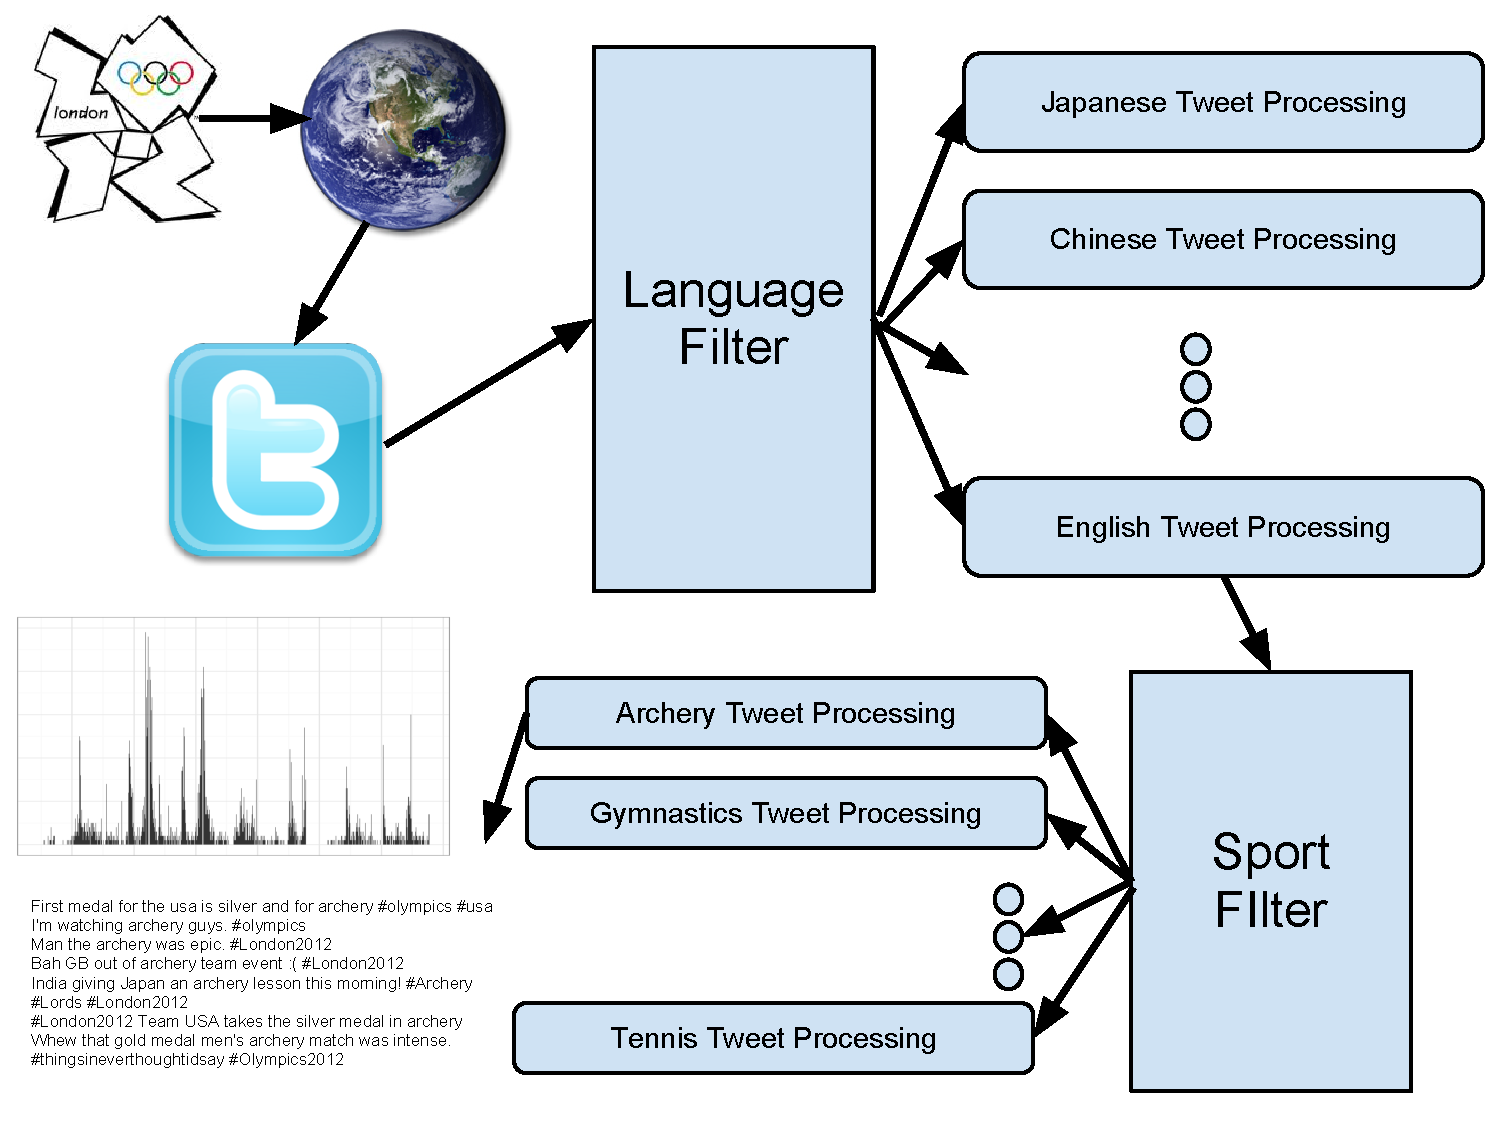
\includegraphics[width=\textwidth,height=.90\textheight]{TweetSummaryModel.pdf}

\end{frame}

\begin{frame}{The Current Realization}

\href{http://fozziethebeat.github.com/tweetolympics/}{\textit{Demo Time}}

\end{frame}

\section{The Tweet Summarization Problem}

\subsection{The General Framework}

\begin{frame}{The General Framework}

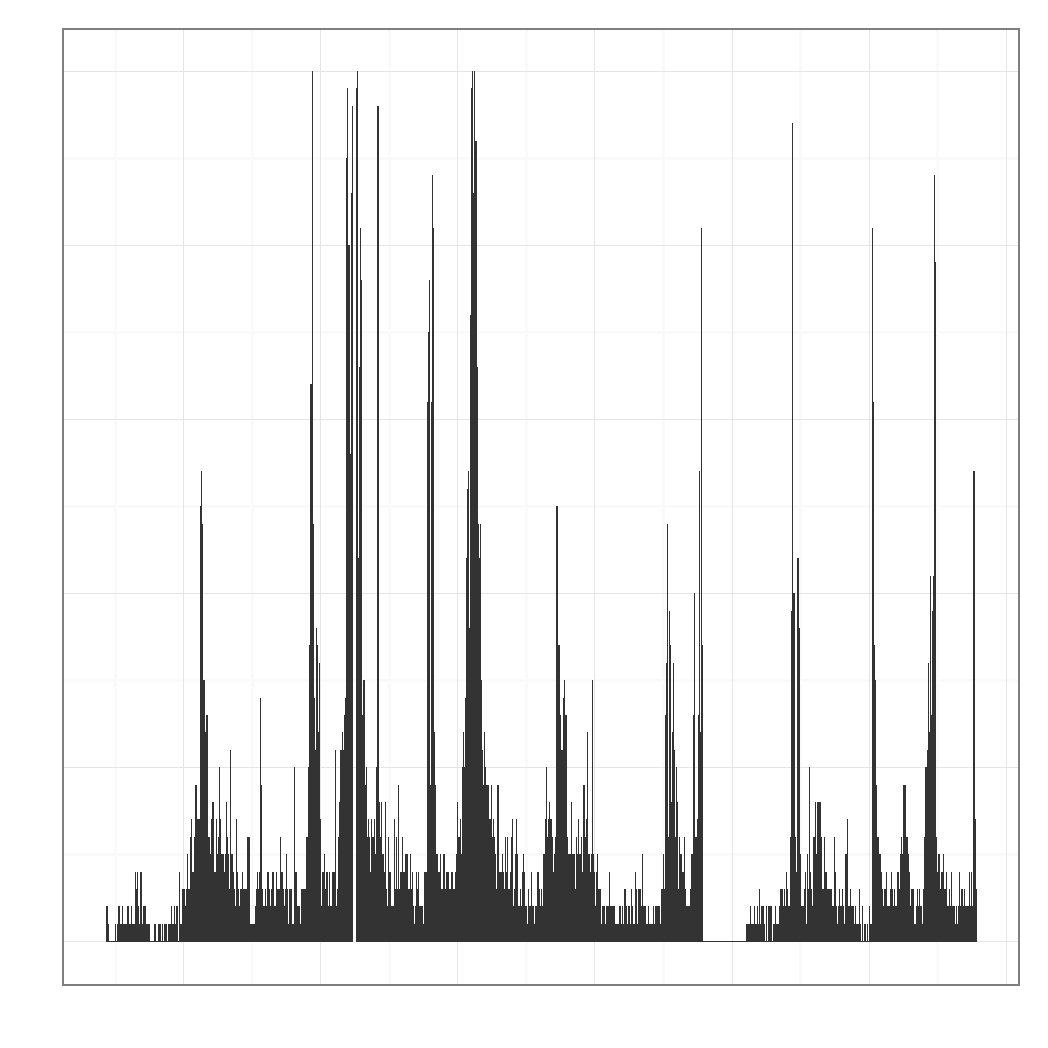
\includegraphics[width=\textwidth,height=.50\textheight]{tweet-archery-example.pdf}

\begin{block}{Summarization Steps}
  \begin{enumerate}
      \item Segment time series of tweets
      \item Find most descriptive summary of each segment
  \end{enumerate}
\end{block}

\end{frame}

\subsection{Segmenting The Time Series}

\begin{frame}{Summarizing the true problem}

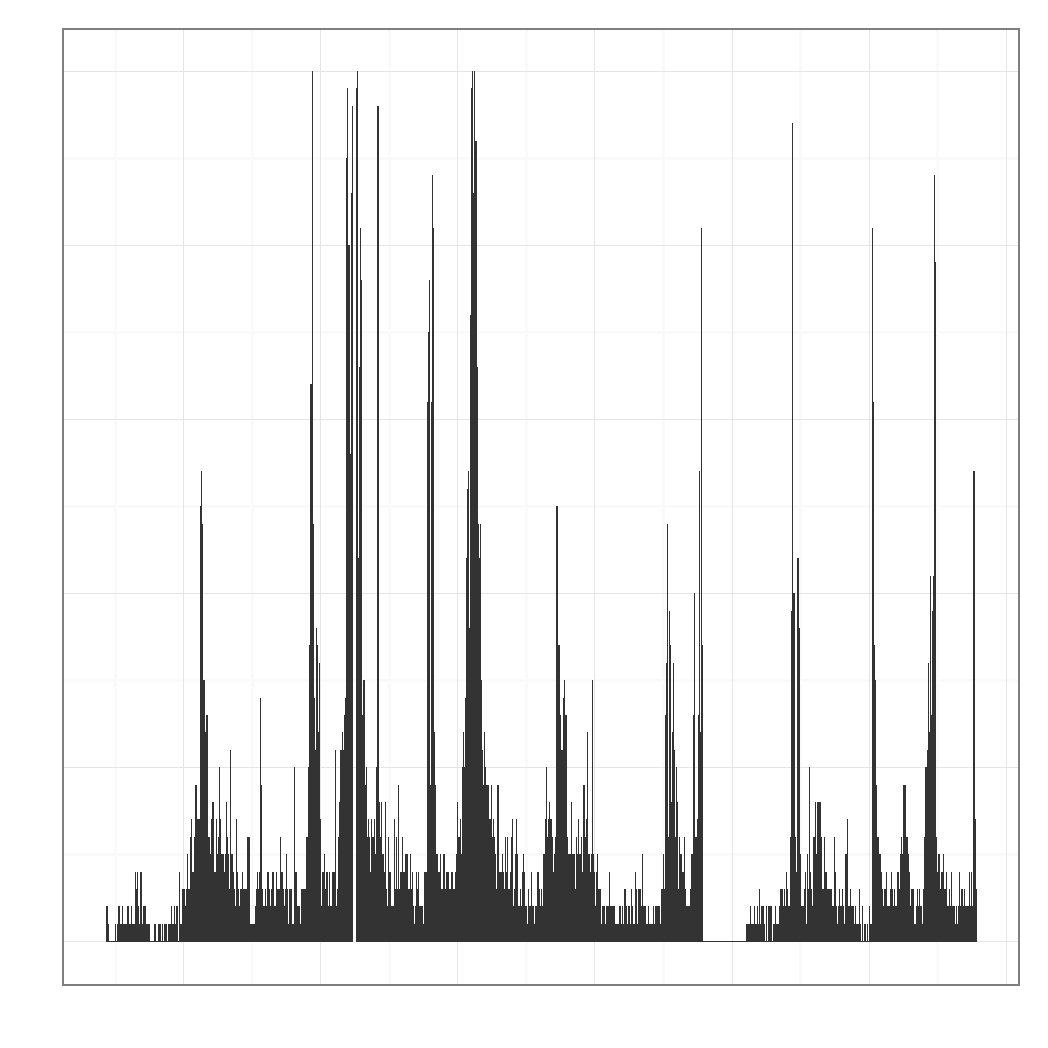
\includegraphics[width=\textwidth,height=.50\textheight]{tweet-archery-example.pdf}

\only<-3>{
\begin{block}{Segmentation goals}
    \begin{enumerate}[<+->]
        \item Segments are ordered along time
        \item Segments represent moments of similar activity
        \item Segmentation is \textit{Change Point Analysis}
    \end{enumerate}
\end{block}
}
\only<4->{
\begin{block}{Segmentation methods}
    \begin{enumerate}[<+->]
        \item The Budgeted Median method \cite{takamura11SummaryStream}
        \item Modified Budgeted Median Method
        \item A basic online Particle Filter
        \item Bayesian on-line changepoint detection \cite{caron11onlineDetection}
    \end{enumerate}
\end{block}
}

\end{frame}

\begin{frame}{The Budgeted Median Method}

\begin{block}{Basic Idea}
Segment the time series by minimizing \textit{conductance}.
\end{block}

\begin{columns}
\begin{column}[1]{3.5cm}
\only<1>{
Original Formulation
\[
\begin{array}{r c l }
max & \sum_{i,j} e_{ij}z_{ij} & \\
s.t. & z_{ij} \leq x_i & \forall i,j \\
& \sum_i x_i \leq p & \\
& \sum_i z_{ij} = 1 & \forall j \\
& z_{ii} = x_i & \forall i \\
& x_i \in \{0,1\} & \forall i \\
& z_{ij} \in \{0,1\} & \forall i,j \\
\end{array}
\]
}
\only<2>{
Similarity Function
\[
sim(x_i, x_j) = \lambda^{|t_i - t_j|/\beta} \frac{x_i \cdot x_j}{|x_i||x_j|}
\]
{\small
\textit{Note:} I'm using cosine similarity between tweets, but many other
metrics like the Jaccard index are equally valid.
}
}
\end{column}
\begin{column}[2]{5cm}
Alternate Formulation
\[
\begin{array}{r c l }
max & \sum_i sim(x_i, \mu_{z_i}) & \\
s.t. & z_{i-1} \leq z_i \leq z_{i+1} & \\
& \mu_j = argmax_{x_i} \sum_{k} sim(x_i, x_k) & \\
& \forall z_i = z_k = j & \\
\end{array}
\]

\end{column}
\end{columns}

\end{frame}

\begin{frame}[fragile]
\frametitle{Solving the Budgeted Median Problem}
\small{
\begin{algorithm}[H]
$\mu_k \leftarrow sample(X)$ \\
sort($\mu$) by $t_k$ \\
$z_k \leftarrow k$ \\
$updated \leftarrow true$ \\
\While{$updated$} {
    \For{$\mu_l,\mu_m \leftarrow \mu.sliding(2)$} {
        $X_r \leftarrow x_i$ s.t. $t_l \leq t_i \leq t_m$ \\
        $b \leftarrow \argmax_{x_p \in X_r} \sum_{i=l}^p sim(x_i, \mu_l) +
                                                   \sum_{i=p+1}^m sim(x_i, \mu_m)$ \\
        $z_{l \leq i \leq p} \leftarrow z_l$ \\
        $z_{p+1 \leq i \leq m} \leftarrow z_m$ \\
    }
    $\mu_k \leftarrow \argmax_{x_j} \sum_{x_i} sim(x_i, x_j)$, s.t. $z_j = z_i = z_k$ \\
    $updated \leftarrow ifChanged(\mu, z)$
}
\end{algorithm}
}
\end{frame}

\begin{frame}{From Medians to Means}

\begin{block}{Key Insight}
Tweets are sparse, therefor $sim(x,y)$ will likely result in $0$.
\end{block}

\pause

Let $\mu_k$ be the \textit{average tweet} within a group.  \\
This makes it a Budgeted Mean problem.

\begin{columns}
\begin{column}[1]{3.5cm}
Similarity Function
\[
sim(x_i, x_j) = \lambda^{|t_i - t_j|/beta} \frac{x_i \cdot x_j}{|x_i||x_j|}
\]
\end{column}
\begin{column}[2]{5cm}
Alternate Formulation
\[
\begin{array}{r c l }
max & \sum_i sim(x_i, \mu_{z_i}) & \\
s.t. & z_{i-1} \leq z_i \leq z_{i+1} & \\
& \mu_j = \frac{sum_{x_i} x_i}{|\{z_i = z_j\}|} & \\
& \forall z_i = z_k = z_j & \\
\end{array}
\]

\end{column}
\end{columns}
General solution remains the same except for how to compute $\mu_k$.
\end{frame}

\begin{frame}{Particle Filtering for segments}
\begin{block}{Ultimate goal}
Develop a streaming algorithm for Budgeted Median/Mean\\
Handle each data point only \textit{once}
\end{block}

\pause

\begin{block}{Particle Filter basics}
\begin{itemize}
    \item Particles represent proposed solutions \\
    \item For each data point
    \begin{enumerate}
        \item Update each particle with new data point
        \item Test the quality of each particle
        \item Filter out poor particles
        \item Generate new particles if needed
    \end{enumerate}
    \item Particles that survive represent most likely solutions.
\end{itemize}
\end{block}

\end{frame}

\begin{frame}{Making the Particle Filter Work}

\begin{block}{Limitations}
\begin{enumerate}
\item No fixed number of segments
\item Any new data point may signify a new segment
\end{enumerate}
\end{block}

\pause

\begin{columns}
\begin{column}[1]{5cm}

\begin{itemize}
\item The Dirichlet Process handles this well
\item Adjust each particle by adding a new segment or updating last existing
segment with new data point
\item Should include a regularization term to limit number of new particles
\end{itemize}
\end{column}

\begin{column}[2]{5cm}

\tiny{
\begin{algorithm}[H]
$particle_k \leftarrow (\theta, \{\})$ \\
\For {$x_i \in X$} {
    \For {$particle_k \in particle$} {
        $w_k \leftarrow n_{last} / (n_{last}+\alpha) * sim(x_i, \mu_{last})$ \\
        $w_k \leftarrow w_k / (w_k + alpha / (n_{last} + \alpha))$ \\
        \If {$coinFlip(w_k) = True$} {
            $\mu_{last} \leftarrow \mu_{last} + x_i$
            $n_{last} \leftarrow n_{last} + 1$
        } \Else {
            $\mu_{last} \leftarrow x_i$
            $n_{last} \leftarrow 1$
        }
    }
    $new\_particle_k \leftarrow Sample(particle)$ \\
    $particle_k \leftarrow new\_particle_k$ \\
}
\end{algorithm}
}
\end{column}
\end{columns}
\end{frame}

\begin{frame}{A Much Better Particle Filter}

\begin{block}{Bayesian On-line Changepoint Analysis \cite{caron11onlineDetection}}
\begin{itemize}
\item Add new particle for potential new segments
\item Weight particles using similarity function and data likelihood
\item Update \textit{parameters} to model
\end{itemize}
\end{block}

Depends on two key distributions:
\begin{columns}

\begin{column}[1]{5cm}
Probability of new assignment:
\[
f(z_i | \mu_l) = \left\{
    \begin{array}{l}
    \frac{1 - H(t_i - t_l - 1)}{1 - H(t_i - t_l - 2)}  \\
    \frac{H(t_i - t_l - 1) - H(t_i - t_l - 2)}{1 - H(t_i - t_l - 2)} 
    \end{array}
    \right.
\]
\end{column}
\begin{column}[2]{5cm}
Probability of data:
\[
g(x_i | z_i) = \left\{
    \begin{array}{l}
    \frac{p(t_{z_i}, t_i)}{p(t_{z_i}, t_{i-1})}  \\
    p(t_i, t_{i-1}) 
    \end{array}
    \right.
\]
\end{column}

\end{columns}

\end{frame}

\begin{frame}{The On-line Bayesian Algorithm}
\begin{algorithm}[H]
$particle^k \leftarrow (\{\})$ \\
\For {$x_i \in X$} {
    $\hat{w}^k \leftarrow g_{\theta}(x_i | z_{i-1}^k) 
                            f_{\theta}(z_{i-1}^k, z_{i-1}^k)$ \\
    $\hat{w}^n \leftarrow g_{\theta}(x_i | i) 
                            \sum_j^K f_{\theta}(i |  z_{i-1}^j) 
                            w^j$ \\

    $\hat{alpha}^k \leftarrow \hat{w}^k 
                              [ \nabla log(g_{\theta}(x_i | z_{i-1}^k))  +
                                \nabla log(f_{\theta}(z_{i-1}^k, z_{i-1}^k))]$ \\
    $\hat{alpha}^n \leftarrow g_{\theta}(x_i | i)
                              (\sum_j^K f_{\theta}(i |  z_{i-1}^j) w^j
                               [ \nabla log( g_{\theta}(x_i | i) ) +
                                 \nabla log(f_{\theta}(i |  z_{i-1}^j))] + 
                                 \beta^j)$ \\
    $\theta = \theta + \gamma \frac{\sum \hat{\alpha}^k}{\sum \hat{w}^k} $\\
    $particle^k = Sample(\hat{w})$ \\
    Update $\beta$ \\
}

\end{algorithm}
\end{frame}

\begin{frame}{Advantages And Disadvantages}
\begin{columns}
\begin{column}[1]{5cm}
Advantages:
\begin{itemize}
\item $g(\cdot)$ allows for any distribution, including one based on our
similarity function.
\item All parameters can be estimated from the data
\item Processing each data point takes constant time
\end{itemize}
\end{column}

\begin{column}[2]{5cm}
Disadvantages:
\begin{itemize}
\item Selecting $H(t)$ and $p(t_i, t_j)$ can be challenging
\item Taking the gradient of $f$ and $g$ can be difficult
\item Implementation is difficult
\item Limited to discrete time steps
\item Relatively new and untested in most domains
\end{itemize}
\end{column}

\end{columns}
\end{frame}

\begin{frame}{HOWEVER!}
\begin{block}{Batch versions of this method exist}
The R $bcp$ package provides an easy to use implementation
\end{block}

% Include screen shot of result of running this on archery and interpret it.

\end{frame}

\subsection{Finding Optimal Summaries}

\begin{frame}[fragile]
\frametitle{Many Paths to summarizing}

{\fontsize{1}{0}\selectfont
\begin{verbatim}
RT @ANCALERTS: #london2012 RT @l2012archery: Men's Individual Ranking Round has ended. View unofficial results #Archery
RT @archeryGlen: Half way through the men's ranking Korea are holding places 1, 2, &amp; 3 TeamGB's Larry Godfrey is hot on their heels ...
Larry's on fire! 680 for the ranking round - great shooting. #archery #london2012 #GoTeamGB
RT @ReutersSports: #London2012 Live Blog: Boris vs Mitt, Usain hangs out, and archery gets underway as the Opening Ceremony draws near h ...
South Korea have claimed the first two world records of #London2012 in the men's archery ranking round. #Olympics
RT @archerynicky: Unofficial 1/2 way teams ranking- 1. Korea 2. France 3. USA. GB currently 5th out of the 12 team #london2012 #archery
why isn't the archery on tv?! #london2012
RT @ReutersSports: #London2012 Live Blog: Boris vs Mitt, Usain hangs out, and archery gets underway as the Opening Ceremony draws near h ...
RT @ANCALERTS: #london2012 RT @l2012archery: Men's Individual Ranking Round has ended. View unofficial results #Archery
Wow. Two World Records set already… South Korea in the archery. #Olympics
“@ANCALERTS: #london2012 RT @l2012archery: Men's Individual Ranking Round has ended. View unofficial results #Archery
RT @TheSunOlympics: South Korea have claimed the first two world records of #London2012 in the men's archery ranking round. #Olympics
The first world records have been set! #London2012 Well done to the Chinese archery team!
First #worldrecord of the #Olympics in the archery apparently #london2012
Great 4th place for Larry Godfrey of #TeamGB in the mens archery ranking round this morning #London2012
Why wouldn't spectators be allowed in to watch the archery? #London2012
Don't forget to keep an eye out for the archery. #Olympics
Brilliant performance GBs Larry Godfrey 4th, Alan Wills 42nd, Simon Terry 50th. Team 8th- very tight #archery #london2012 #expertsnetwork
100s of people turned away from Olympics archery event at Lords's because of ticket confusion. Smh....#London2012
\end{verbatim}
}

\pause

\begin{block}{}
    \begin{enumerate}[<+->]
        \item Select the median of the segment \cite{takamura11SummaryStream}
        \item Select the most average 
        \item Select the sentence with best phrases \cite{nichols12SummarySports}
    \end{enumerate}
\end{block}

\end{frame}

\begin{frame}{Selecting the Median/Mean tweet}
\begin{block}{Basic Intuition}
The representative tweet for a segment also represents the summary of the segment
\end{block}

\begin{columns}

\begin{column}[1]{5cm}
The Median Tweet:
\[
\begin{array}{l l}
\argmax_{x_i} \sum_{x_j} sim(x_i, x_j) \\
\text{s.t. } z_i = z_j \\
\end{array}
\]
\end{column}

\begin{column}[2]{5cm}
The Mean Tweet:
\[
\begin{array}{l l}
\mu_k = \frac{\sum_{x_i} x_i}{|\{z_i = z_k\}|} \\
\argmax_{x_i} sim(x_i, \mu_k) \\
\text{s.t. } z_i = z_j = z_k \\
\end{array}
\]
\end{column}

\end{columns}

\end{frame}

\begin{frame}{Selection using a phrase graph}
\begin{block}{Basic Motivation}
Mean/Median summary methods ignore word ordering or presence of strong phrases
\end{block}
\pause
Solution: Build a large Phrase Graph
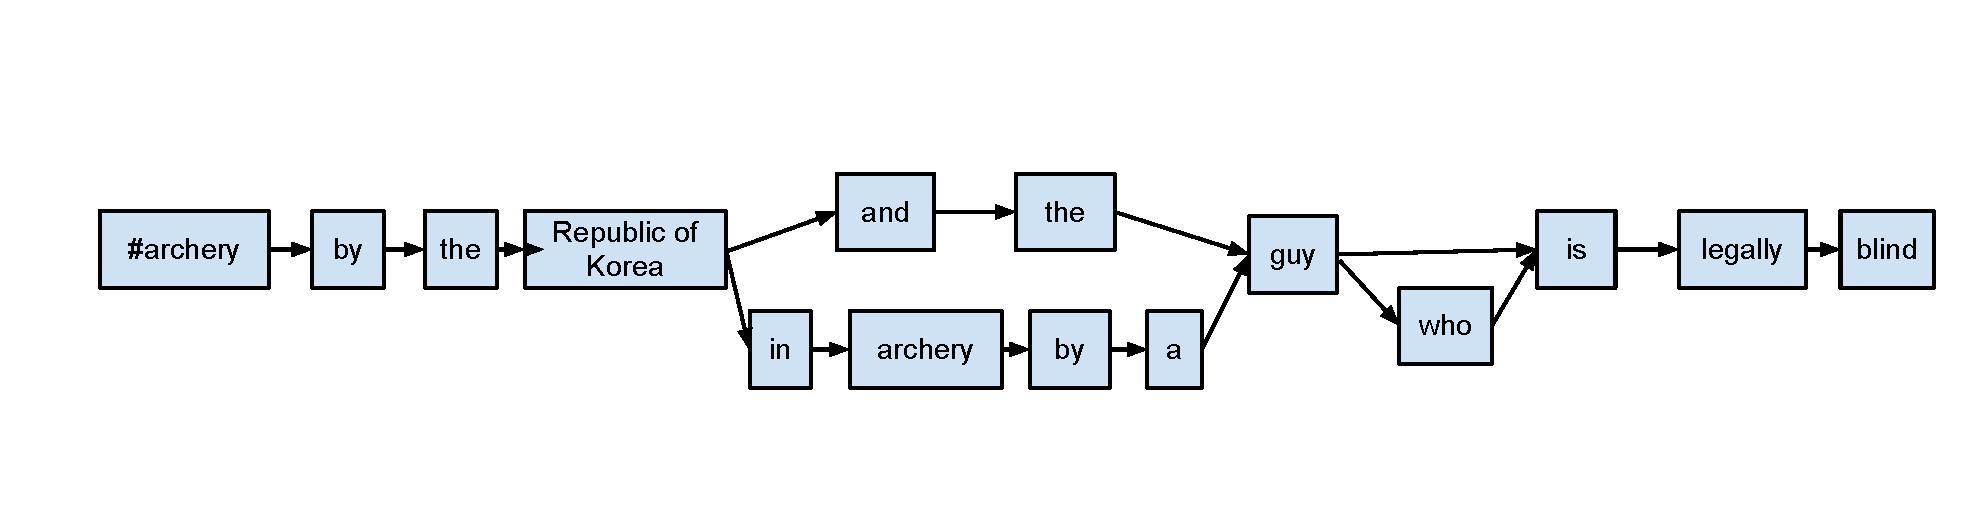
\includegraphics[width=\textwidth,height=.50\textheight]{example-phrase-graph.pdf}
\end{frame}

\begin{frame}{How to build a phrase graph}
\begin{block}{Basic Goals}
\begin{itemize}
\item Weighted Nodes represent tokens with frequencies
\item Directed paths represent full phrases
\item Key Phrases should have high path weights
\end{itemize}
\end{block}

\pause

\begin{columns}
\begin{column}[1]{5cm}
Formally: \\
A Weighted Minimal Acyclic Finite-State Automata \\
Like a Trie, but compressed at both ends \\
With extra compression in the middle \\
\pause
\end{column}
\begin{column}[2]{5cm}
Construction Algorithm\cite{daciuk99incremental}:
{\tiny
\begin{algorithm}[H]
Lexicographically sort $Tweets$ \\
\For {$tweet \in Tweets$} {
    $(prefixMatch, suffix) \leftarrow walk(tweet)$ \\
    $lastState \leftarrow tail(prefixMatch)$ \\
    \If {$lastState.hasChildren$} {
        $replace\_or\_register(lastState)$
    }
    $add(lastState, suffix)$ \\
}
$replace\_or\_register(root)$
\end{algorithm}
}

\end{column}
\end{columns}
\end{frame}

\section{Results}
\subsection{Segmentation Results}

\begin{frame}{Testing the segmentation algorithms}
\begin{block}{Simple Evaluation: Do segments line up with event listings?}
\begin{itemize}
\item We may not have detailed listings of game level events, but we know when
each competition took place
\item Compare competition times to discovered segment boundaries
\item Better algorithms should have boundaries closer to competition times
\end{itemize}
\end{block}

\begin{table}[h!t!b!]
\center
\tiny
\begin{tabular}{|c|c|c|c|c|}
\hline
Sport & batch-mean & batch-median & particle-mean & bcp \\
\hline
gymnastics & \textbf{7807} & 8578 & 18598 & 155030 \\
fencing & 81125 & 79869 & \textbf{73987} & 12509093 \\
tennis & 91205 & 92450 & \textbf{80067} & 933588 \\
archery & \textbf{64468} & 76734 & 69980 & 586340 \\
judo & 116757 & \textbf{112873} & 153348 & 1759213 \\
\hline
\end{tabular}

\caption{Total Absolute Error between nearest discovered segment and known
competition times}
\end{table}

\end{frame}

\subsection{Summarization Results}
\begin{frame}{Finding differences between summary methods}
\end{frame}

\section{Deeper thoughts}
\subsection{Handling Twitter}
\begin{frame}{Observations from Twitter}
\end{frame}

\section{Bibliography}

\begin{frame}
\bibliographystyle{acm}
\bibliography{presentation}
\end{frame}

\end{document}
